\newpage
\subsection{Validazione e collaudo}
Questo periodo inizia il giorno dopo la  \textit{Revisione di Qualifica}(20/04/2019) e si conclude con la consegna dei documenti per la  \textit{Revisione di Accettazione}(10/05/2019). 
\begin{itemize}
	\item{\textbf{Incremento e Verifica:} all’inizio del periodo vengono svolte attività di Incremento e Verifica su vari documenti;}
	\item{\textbf{Glossario:} questa attività comprende sia il miglioramento del Glossario che l’aggiunta dei nuovi termini;}
	\item{\textbf{Validazione e Collaudo:} questa attività consiste nell'attuare vari ed ulteriori test al fine di assicurare la massima qualità conforme agli obiettivi richiesti;}
	\item{\textbf{Manuale Utente:} questa attività consiste nel miglioramento e completamento del \textit{Manuale utente}, contenente indicazioni sull’utilizzo dell’applicazione.}
\end{itemize}

\clearpage
\begin{figure}[!htpb]
	\centering
	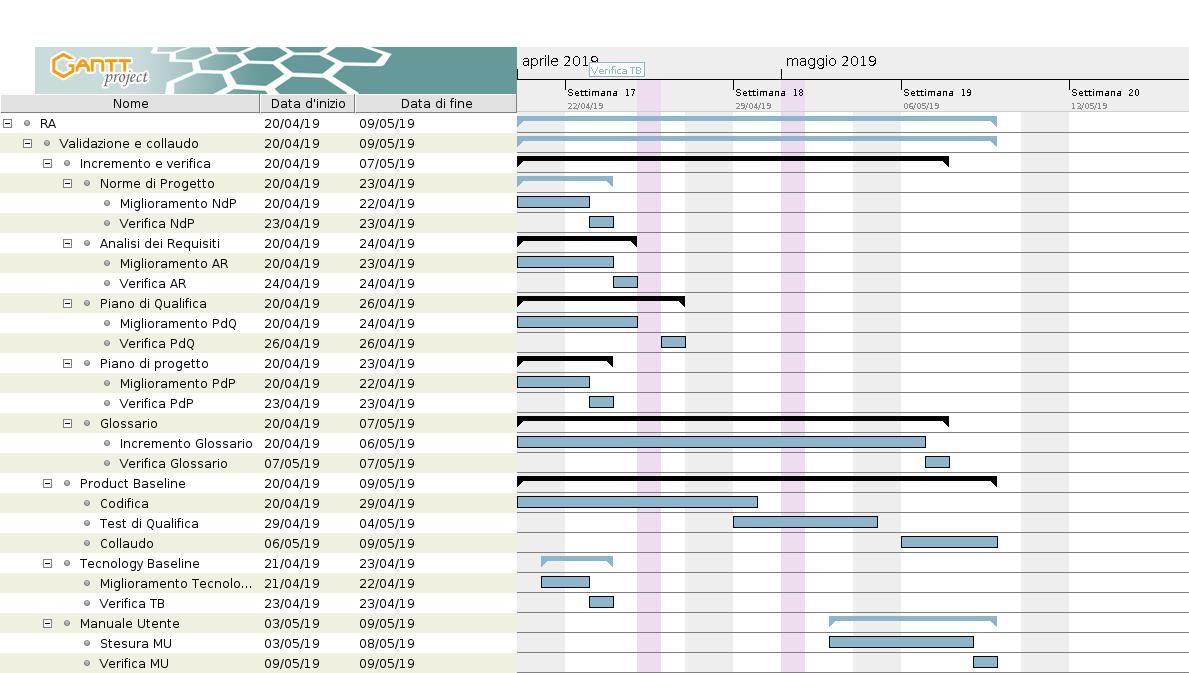
\includegraphics[width=0.8\textwidth]{gantcollaudo.jpg}
	\caption{Diagramma di Gantt del periodo di Validazione e collaudo}
\end{figure}

\begin{figure}[!htpb]
	\centering
	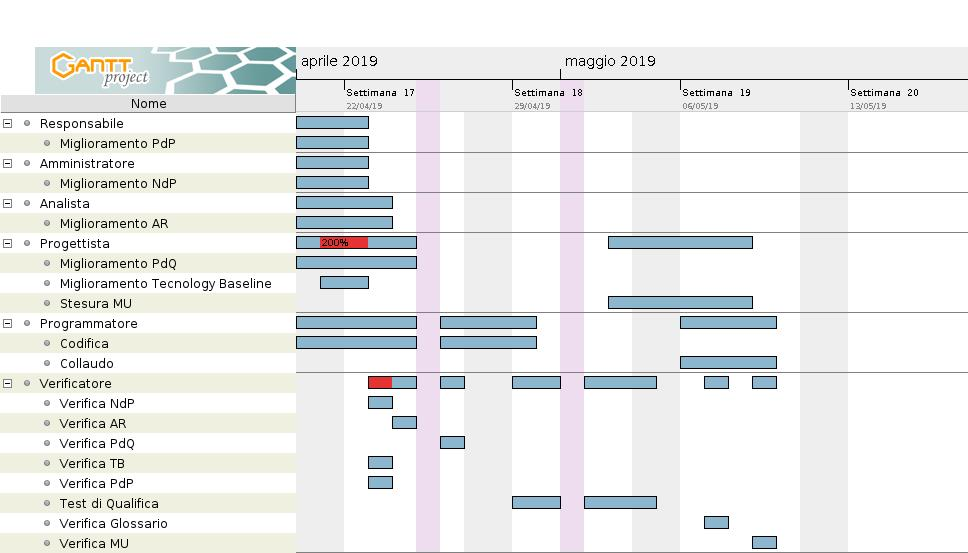
\includegraphics[width=0.8\textwidth]{gantcollaudorisorse.jpg}
	\caption{Diagramma di Gantt del periodo di Validazione e collaudo}
\end{figure}

\begin{table}[!htpb]
	\centering
	\renewcommand{\arraystretch}{2} 
	\rowcolors{2}{gray!25}{white}
	\begin{tabular}{|l|p{5cm}|p{5cm}|}
		\rowcolor{orange!50}
		\hline
		\multicolumn{3}{|c|}{\textbf{Suddivisione temporale}}\\
		\hline
		\textbf{Ruolo} & \textbf{20/04/19 - 29/04/19} & \textbf{29/04/19 - 10/05/19} \\
		\hline
		\textbf{Responsabile} & \gia  & \daG   \\
		\hline
		\textbf{Amministratore} & \pie & \mat \\
		\hline
		\textbf{Analista} & - & - \\
		\hline
		\textbf{Progettista} & - & - \\
		\hline
		\textbf{Programmatore} & \mar & \mic \\
		\hline
		\textbf{Verificatore} & \parbox{5cm}{\mat \\ \mic \\ \daG \\ \daL} & \parbox{5cm}{\daL \\ \pie \\ \gia \\ \mar}\\
		\hline
	\end{tabular}
	\caption{Suddivisione temporale del periodo di Validazione e collaudo}
\end{table}
	
